\documentclass[11pt]{article}

\usepackage[utf8]{inputenc}
\usepackage[T1]{fontenc}
\usepackage{mathptmx}
\usepackage[margin=1in]{geometry}
\usepackage{url}
\urlstyle{same}
\usepackage{graphicx}
\usepackage{booktabs}
\usepackage{array}
\usepackage{amsmath}
\usepackage[font=small,labelfont=bf]{caption}
\usepackage[hidelinks]{hyperref}

% Every \lhd macro prints a number computed from the saved runs. numbers.tex lists each one with its source.
% Written by experiments/paper_short.py from the saved runs. Rebuild it, never edit it.
\newcommand{\lhdRuns}{885}% runs in total [results/tables/run_counts.csv]
\newcommand{\lhdCalibrationRuns}{60}% calibration runs, all networks [results/summary.json]
\newcommand{\lhdCalibrationPerNet}{20}% calibration runs per network [experiments/grid.py]
\newcommand{\lhdFreshRuns}{150}% fresh healthy runs, all networks [results/summary.json]
\newcommand{\lhdBrokenRuns}{470}% broken runs with a frozen layer or dead units [results/summary.json]
\newcommand{\lhdOtherRuns}{205}% runs with the extra faults (third set) [results/summary.json]
\newcommand{\lhdCaught}{411}% broken runs LHD caught [results/summary.json]
\newcommand{\lhdCaughtRate}{87\%}% share of broken runs LHD caught [results/summary.json]
\newcommand{\lhdCaughtInterval}{84 to 90\%}% 95% Wilson interval of that share [results/summary.json]
\newcommand{\lhdAccCaught}{166}% broken runs the accuracy curve caught [results/summary.json]
\newcommand{\lhdAccCaughtRate}{35\%}% share the accuracy curve caught [results/summary.json]
\newcommand{\lhdMedianEpoch}{3}% median epoch of LHD's alarm [results/summary.json]
\newcommand{\lhdAccMedianEpoch}{6}% median epoch of the accuracy curve's alarm [results/summary.json]
\newcommand{\lhdAccNever}{61\%}% runs LHD caught that the accuracy curve never caught [results/summary.json]
\newcommand{\lhdSilentShare}{66\%}% broken runs whose final accuracy ended inside the healthy range [results/summary.json]
\newcommand{\lhdBothCaught}{162}% broken runs both LHD and the accuracy curve caught [results/tables/runs.csv]
\newcommand{\lhdBothGap}{4.6}% mean epochs LHD was earlier on those runs [results/tables/runs.csv]
\newcommand{\lhdBothMedian}{3}% median epochs LHD was earlier on those runs [results/tables/runs.csv]
\newcommand{\lhdBothAccEarlier}{1}% of those runs, accuracy curve earlier [results/tables/runs.csv]
\newcommand{\lhdBothTies}{26}% of those runs, same epoch [results/tables/runs.csv]
\newcommand{\lhdLayerRight}{98.1\%}% caught runs where LHD named the planted layer [results/summary.json]
\newcommand{\lhdLayerRightRuns}{403 of 411}% the same as runs [results/summary.json]
\newcommand{\lhdCauseRight}{96.8\%}% caught runs where LHD named the planted cause [results/summary.json]
\newcommand{\lhdCauseRightRuns}{398 of 411}% the same as runs [results/summary.json]
\newcommand{\lhdFalseAlarms}{3}% fresh healthy runs LHD flagged [results/summary.json]
\newcommand{\lhdHealthyRuns}{150}% fresh healthy runs scored [results/summary.json]
\newcommand{\lhdFalseAlarmRate}{2.0\%}% LHD false alarm rate [results/summary.json]
\newcommand{\lhdFalseAlarmInterval}{0.7 to 5.7\%}% 95% Wilson interval of that rate [results/summary.json]
\newcommand{\lhdAccFalseAlarms}{7}% fresh healthy runs the accuracy curve flagged [results/summary.json]
\newcommand{\lhdAccFalseAlarmInterval}{2.3 to 9.3\%}% 95% Wilson interval of that rate [results/summary.json]
\newcommand{\lhdSeedGroups}{30}% seed groups (network and seed) [results/summary.json]
\newcommand{\lhdSeedGroupsLHD}{30}% seed groups whose mean gap favored LHD [results/summary.json]
\newcommand{\lhdSeedP}{$p = 9.3 \times 10^{-10}$}% one sided Wilcoxon over seed groups [results/summary.json]
\newcommand{\lhdConditions}{47}% fault conditions (network, fault, layer) [results/tables/runs.csv]
\newcommand{\lhdConditionsLHD}{41}% conditions whose mean gap favored LHD [results/tables/runs.csv]
\newcommand{\lhdConditionsAcc}{3}% conditions where the accuracy curve was earlier [results/tables/runs.csv]
\newcommand{\lhdConditionsSame}{1}% conditions where both fired at the same epoch [results/tables/runs.csv]
\newcommand{\lhdConditionsNeither}{2}% conditions where neither fired [results/tables/runs.csv]
\newcommand{\lhdConditionP}{$p < 10^{-10}$}% one sided Wilcoxon over conditions [results/summary.json]
\newcommand{\lhdMeanGapAll}{9.1}% mean gap over all broken runs, never as one past the end [results/summary.json]
\newcommand{\lhdMeanGapInterval}{8.4 to 9.7}% 95% bootstrap interval over seeds [results/summary.json]
\newcommand{\lhdHarmSmall}{223}% broken runs whose fault cost under 0.5 pts [results/tables/harm.csv]
\newcommand{\lhdHarmSmallLHD}{186}% of those, LHD caught [results/tables/harm.csv]
\newcommand{\lhdHarmSmallAcc}{33}% of those, the accuracy curve caught [results/tables/harm.csv]
\newcommand{\lhdHarmMid}{142}% broken runs whose fault cost 0.5 to 2 pts [results/tables/harm.csv]
\newcommand{\lhdHarmMidLHD}{131}% of those, LHD caught [results/tables/harm.csv]
\newcommand{\lhdHarmMidAcc}{73}% of those, the accuracy curve caught [results/tables/harm.csv]
\newcommand{\lhdHarmBig}{105}% broken runs whose fault cost 2 pts or more [results/tables/harm.csv]
\newcommand{\lhdHarmBigLHD}{94}% of those, LHD caught [results/tables/harm.csv]
\newcommand{\lhdHarmBigAcc}{60}% of those, the accuracy curve caught [results/tables/harm.csv]
\newcommand{\lhdCnnFrozenDrop}{11.1}% mean accuracy points a frozen CNN layer cost against the twin [results/tables/runs.csv]
\newcommand{\lhdCnnHalfDeadDrop}{3.1}% mean points half a CNN layer's units dead cost [results/tables/runs.csv]
\newcommand{\lhdOtherMaxDrop}{0.8}% largest mean cost of any fault in the other two networks [results/tables/runs.csv]
\newcommand{\lhdLhdFrozenRight}{97\%}% frozen layers LHD caught at the planted layer [results/tables/detectors.csv]
\newcommand{\lhdLhdDeadRight}{78\%}% dead unit faults LHD caught at the planted layer [results/tables/detectors.csv]
\newcommand{\lhdLhdDeadAny}{78\%}% dead unit faults LHD caught at any layer [results/tables/detectors.csv]
\newcommand{\lhdZeroFrozen}{100\%}% Zero update check, frozen layers caught at the planted layer [results/tables/detectors.csv]
\newcommand{\lhdZeroDead}{0\%}% Zero update check, dead unit faults caught at the planted layer [results/tables/detectors.csv]
\newcommand{\lhdZeroFlagged}{0}% Zero update check, healthy runs flagged (of 150) [results/tables/detectors.csv]
\newcommand{\lhdQuarterFrozen}{0\%}% 25% dead rule, frozen layers caught at the planted layer [results/tables/detectors.csv]
\newcommand{\lhdQuarterDead}{71\%}% 25% dead rule, dead unit faults caught at the planted layer [results/tables/detectors.csv]
\newcommand{\lhdQuarterFlagged}{51}% 25% dead rule, healthy runs flagged (of 150) [results/tables/detectors.csv]
\newcommand{\lhdSageFrozen}{0\%}% SageMaker Debugger (50%), frozen layers caught at the planted layer [results/tables/detectors.csv]
\newcommand{\lhdSageDead}{40\%}% SageMaker Debugger (50%), dead unit faults caught at the planted layer [results/tables/detectors.csv]
\newcommand{\lhdSageFlagged}{22}% SageMaker Debugger (50%), healthy runs flagged (of 150) [results/tables/detectors.csv]
\newcommand{\lhdDeepFrozen}{0\%}% DeepDiagnosis (70%), frozen layers caught at the planted layer [results/tables/detectors.csv]
\newcommand{\lhdDeepDead}{4\%}% DeepDiagnosis (70%), dead unit faults caught at the planted layer [results/tables/detectors.csv]
\newcommand{\lhdDeepFlagged}{0}% DeepDiagnosis (70%), healthy runs flagged (of 150) [results/tables/detectors.csv]
\newcommand{\lhdWandbFrozen}{0\%}% wandb-callbacks (80%), frozen layers caught at the planted layer [results/tables/detectors.csv]
\newcommand{\lhdWandbDead}{0\%}% wandb-callbacks (80%), dead unit faults caught at the planted layer [results/tables/detectors.csv]
\newcommand{\lhdWandbFlagged}{0}% wandb-callbacks (80%), healthy runs flagged (of 150) [results/tables/detectors.csv]
\newcommand{\lhdAnyDeadFrozen}{2\%}% Any dead unit (wandb-callbacks verbose), frozen layers caught at the planted layer [results/tables/detectors.csv]
\newcommand{\lhdAnyDeadDead}{74\%}% Any dead unit (wandb-callbacks verbose), dead unit faults caught at the planted layer [results/tables/detectors.csv]
\newcommand{\lhdAnyDeadFlagged}{100}% Any dead unit (wandb-callbacks verbose), healthy runs flagged (of 150) [results/tables/detectors.csv]
\newcommand{\lhdZeroFrozenRuns}{200 of 200}% frozen layers the zero update check caught at the planted layer [results/tables/detectors.csv]
\newcommand{\lhdZeroFrozenOneEpoch}{200 of 200}% the same check when one epoch is enough [results/tables/detectors.csv]
\newcommand{\lhdZeroEpoch}{1}% median epoch of that one epoch check [results/tables/detectors.csv]
\newcommand{\lhdLhdFrozenEpoch}{3}% median epoch of LHD's alarm on frozen layers [results/tables/detectors.csv]
\newcommand{\lhdZeroLead}{2}% epochs the zero update check fires before LHD [results/tables/detectors.csv]
\newcommand{\lhdPatienceAlarmChange}{0}% largest change in false alarms between one and three epochs, fixed rules [results/tables/detectors.csv]
\newcommand{\lhdPatienceDeadChange}{2}% largest drop in dead unit catches between one and three epochs [results/tables/detectors.csv]
\newcommand{\lhdSageAnyTen}{26}% 50% rule catches of 10% dead units at any layer [results/tables/detectors.csv]
\newcommand{\lhdSageRightTen}{8}% 50% rule catches of 10% dead units at the planted layer [results/tables/detectors.csv]
\newcommand{\lhdSageAnyTwentyFive}{25}% 50% rule catches of 25% dead units at any layer [results/tables/detectors.csv]
\newcommand{\lhdSageRightTwentyFive}{10}% 50% rule catches of 25% dead units at the planted layer [results/tables/detectors.csv]
\newcommand{\lhdCnnDenseLow}{36\%}% fewest dead units in the CNN's fc1, calibration runs [results/tables/signals.csv.gz]
\newcommand{\lhdCnnDenseHigh}{70\%}% most dead units in the CNN's fc1, calibration runs [results/tables/signals.csv.gz]
\newcommand{\lhdTransformerDeadMax}{0\%}% most dead units in any transformer ReLU layer, calibration [results/tables/signals.csv.gz]
\newcommand{\lhdAlarmARun}{mlp-fresh-none-s1046}% false alarm run [results/tables/false_alarms.csv]
\newcommand{\lhdAlarmALayer}{fc2}% layer it named [results/tables/false_alarms.csv]
\newcommand{\lhdAlarmAEpoch}{16}% epoch it fired [results/tables/false_alarms.csv]
\newcommand{\lhdAlarmASignal}{dead unit fraction}% signal out of range [results/tables/false_alarms.csv]
\newcommand{\lhdAlarmAValue}{1.6\%}% dead units in that layer at the alarm [results/tables/signals.csv.gz]
\newcommand{\lhdAlarmAEdge}{3.9\%}% calibration lowest for that layer, so the alarm is below [results/tables/signals.csv.gz]
\newcommand{\lhdAlarmBRun}{cnn-fresh-none-s1015}% false alarm run [results/tables/false_alarms.csv]
\newcommand{\lhdAlarmBLayer}{conv2}% layer it named [results/tables/false_alarms.csv]
\newcommand{\lhdAlarmBEpoch}{4}% epoch it fired [results/tables/false_alarms.csv]
\newcommand{\lhdAlarmBSignal}{dead unit fraction}% signal out of range [results/tables/false_alarms.csv]
\newcommand{\lhdAlarmBValue}{6.2\%}% dead units in that layer at the alarm [results/tables/signals.csv.gz]
\newcommand{\lhdAlarmBEdge}{0.0\%}% calibration highest for that layer, so the alarm is above [results/tables/signals.csv.gz]
\newcommand{\lhdAlarmCRun}{cnn-fresh-none-s1028}% false alarm run [results/tables/false_alarms.csv]
\newcommand{\lhdAlarmCLayer}{conv2}% layer it named [results/tables/false_alarms.csv]
\newcommand{\lhdAlarmCEpoch}{3}% epoch it fired [results/tables/false_alarms.csv]
\newcommand{\lhdAlarmCSignal}{dead unit fraction}% signal out of range [results/tables/false_alarms.csv]
\newcommand{\lhdAlarmCValue}{6.2\%}% dead units in that layer at the alarm [results/tables/signals.csv.gz]
\newcommand{\lhdAlarmCEdge}{0.0\%}% calibration highest for that layer, so the alarm is above [results/tables/signals.csv.gz]
\newcommand{\lhdFloor}{0.05}% floor f [experiments/evaluate.py]
\newcommand{\lhdSmallLayerUnits}{16}% units in the CNN's conv2 [experiments/models.py]
\newcommand{\lhdOneUnitShare}{6.25\%}% one dead unit in that layer [experiments/models.py]
\newcommand{\lhdMargin}{0.5}% margin m [experiments/evaluate.py]
\newcommand{\lhdPatience}{3}% patience p, epochs in a row [experiments/evaluate.py]
\newcommand{\lhdProbeSize}{256}% validation examples in the probe batch [experiments/data.py]
\newcommand{\lhdSettingsCommit}{e83806f}% commit that fixed m, f, and p [experiments/paper.py]
\newcommand{\lhdSettingsDate}{31 October 2026}% date of that commit [git log]
\newcommand{\lhdDivergenceFired}{0}% runs where the divergence rule fired, all faults [results/summary.json]
\newcommand{\lhdVanishingFired}{35}% runs named vanishing gradient, extra faults only [results/summary.json]
\newcommand{\lhdRunawayFired}{5}% runs named runaway weights, extra faults only [results/summary.json]
\newcommand{\lhdMlpParams}{242,762}% parameters, fully connected network [results/tables/networks.csv]
\newcommand{\lhdMlpEpochs}{20}% epochs, fully connected network [experiments/train.py]
\newcommand{\lhdMlpFresh}{50}% fresh healthy runs, fully connected network [results/summary.json]
\newcommand{\lhdMlpBroken}{130}% broken runs in the main study, fully connected network [results/summary.json]
\newcommand{\lhdMlpOther}{55}% runs with extra faults, fully connected network [results/summary.json]
\newcommand{\lhdTransformerParams}{112,577}% parameters, transformer [results/tables/networks.csv]
\newcommand{\lhdTransformerEpochs}{15}% epochs, transformer [experiments/train.py]
\newcommand{\lhdTransformerFresh}{50}% fresh healthy runs, transformer [results/summary.json]
\newcommand{\lhdTransformerBroken}{170}% broken runs in the main study, transformer [results/summary.json]
\newcommand{\lhdTransformerOther}{85}% runs with extra faults, transformer [results/summary.json]
\newcommand{\lhdCnnParams}{41,659}% parameters, CNN [results/tables/networks.csv]
\newcommand{\lhdCnnEpochs}{15}% epochs, CNN [experiments/train.py]
\newcommand{\lhdCnnFresh}{50}% fresh healthy runs, CNN [results/summary.json]
\newcommand{\lhdCnnBroken}{170}% broken runs in the main study, CNN [results/summary.json]
\newcommand{\lhdCnnOther}{65}% runs with extra faults, CNN [results/summary.json]
\newcommand{\lhdMlpWidths}{256, 128, and 64}% hidden widths of the fully connected network [experiments/models.py]
\newcommand{\lhdCnnFilters}{8, 16, and 32}% filters in the CNN's three convolutions [experiments/models.py]
\newcommand{\lhdCnnDense}{64}% units in the CNN's dense layer [experiments/models.py]
\newcommand{\lhdTransformerWidth}{64}% transformer width [experiments/models.py]
\newcommand{\lhdTransformerHeads}{4}% transformer heads [experiments/models.py]
\newcommand{\lhdTransformerBlocks}{2}% transformer depth [experiments/models.py]
\newcommand{\lhdTransformerHidden}{256}% transformer hidden [experiments/models.py]
\newcommand{\lhdCnnValImages}{4,000}% CNN validation images [experiments/train.py]
\newcommand{\lhdTextWindows}{512}% transformer validation windows [experiments/data.py]
\newcommand{\lhdTextContext}{64}% characters per window [experiments/train.py]
\newcommand{\lhdTextHeldOut}{10\%}% share of the text held out for validation [experiments/data.py]
\newcommand{\lhdLearningRate}{0.001}% Adam learning rate [experiments/train.py]
\newcommand{\lhdThreads}{1}% CPU threads per run [experiments/train.py]
\newcommand{\lhdCalibrationSeeds}{0 to 19}% calibration seeds [experiments/grid.py]
\newcommand{\lhdScoredSeedStart}{1000}% first seed of scored runs [experiments/grid.py]
\newcommand{\lhdSeedsPerFault}{10}% seeds per fault condition [experiments/grid.py]
\newcommand{\lhdDeadFractions}{10\%, 25\%, and 50\%}% dead unit shares planted [experiments/grid.py]
\newcommand{\lhdDeadBias}{$-1$}% bias given to killed units [experiments/train.py]
\newcommand{\lhdUnitSeedOffset}{7919}% added to the run's seed to pick the killed units [experiments/train.py]
\newcommand{\lhdDeadChecks}{25\%, 50\%, 70\%, and 80\%}% fixed dead unit thresholds scored [experiments/evaluate.py]
\newcommand{\lhdFreshFirstSet}{90}% fresh healthy runs in the first set [results/tables/runs.csv]
\newcommand{\lhdFreshThirdSet}{60}% fresh healthy runs in the third set [results/tables/runs.csv]
\newcommand{\lhdPlanCommit}{b6bfb6a}% commit with the run plan [experiments/paper.py]
\newcommand{\lhdPlanDate}{31 October 2026}% date of that commit [git log]
\newcommand{\lhdDraftCommit}{d3f5275}% commit of the earlier draft [experiments/paper.py]
\newcommand{\lhdDraftFresh}{110}% fresh healthy runs done at that draft [experiments/paper.py]
\newcommand{\lhdDraftAlarms}{3}% false alarms that draft reported [experiments/paper.py]
\newcommand{\lhdLaterFresh}{40}% fresh healthy runs finished after that draft [results/tables/runs.csv]
\newcommand{\lhdLaterAlarms}{0}% false alarms those later runs added [results/summary.json]
\newcommand{\lhdEpochRange}{15 to 20}% epochs per run [experiments/train.py]
\newcommand{\lhdTransformerAcc}{37\%}% mean final next character accuracy of fresh transformer runs [results/tables/runs.csv]
\newcommand{\lhdCnnDenseACaught}{0 of 10}% CNN fc1 runs with 10% dead units that LHD caught [results/tables/per_layer.csv]
\newcommand{\lhdCnnDenseBCaught}{0 of 10}% CNN fc1 runs with 25% dead units that LHD caught [results/tables/per_layer.csv]
\newcommand{\lhdCnnDenseCCaught}{1 of 10}% CNN fc1 runs with 50% dead units that LHD caught [results/tables/per_layer.csv]
\newcommand{\lhdCalARuns}{2}% calibration runs used to build the range [results/tables/sweep_calibration.csv]
\newcommand{\lhdCalAWorst}{22\%}% highest mean false alarm rate over networks at that size [results/tables/sweep_calibration.csv]
\newcommand{\lhdCalANet}{CNN}% network with that rate [results/tables/sweep_calibration.csv]
\newcommand{\lhdCalBRuns}{3}% calibration runs used to build the range [results/tables/sweep_calibration.csv]
\newcommand{\lhdCalBWorst}{15\%}% highest mean false alarm rate over networks at that size [results/tables/sweep_calibration.csv]
\newcommand{\lhdCalBNet}{CNN}% network with that rate [results/tables/sweep_calibration.csv]
\newcommand{\lhdCalCRuns}{5}% calibration runs used to build the range [results/tables/sweep_calibration.csv]
\newcommand{\lhdCalCWorst}{11\%}% highest mean false alarm rate over networks at that size [results/tables/sweep_calibration.csv]
\newcommand{\lhdCalCNet}{fully connected network}% network with that rate [results/tables/sweep_calibration.csv]
\newcommand{\lhdCalDRuns}{10}% calibration runs used to build the range [results/tables/sweep_calibration.csv]
\newcommand{\lhdCalDWorst}{5\%}% highest mean false alarm rate over networks at that size [results/tables/sweep_calibration.csv]
\newcommand{\lhdCalDNet}{fully connected network}% network with that rate [results/tables/sweep_calibration.csv]
\newcommand{\lhdCalERuns}{15}% calibration runs used to build the range [results/tables/sweep_calibration.csv]
\newcommand{\lhdCalEWorst}{4\%}% highest mean false alarm rate over networks at that size [results/tables/sweep_calibration.csv]
\newcommand{\lhdCalENet}{CNN}% network with that rate [results/tables/sweep_calibration.csv]
\newcommand{\lhdCalFRuns}{20}% calibration runs used to build the range [results/tables/sweep_calibration.csv]
\newcommand{\lhdCalFWorst}{4\%}% highest mean false alarm rate over networks at that size [results/tables/sweep_calibration.csv]
\newcommand{\lhdCalFNet}{CNN}% network with that rate [results/tables/sweep_calibration.csv]
\newcommand{\lhdAccOneCaught}{291 of 470}% Accuracy curve, 1 epoch below healthy, broken runs caught [results/tables/detectors.csv]
\newcommand{\lhdAccOneFlagged}{44 of 150}% Accuracy curve, 1 epoch below healthy, healthy runs flagged [results/tables/detectors.csv]
\newcommand{\lhdLossCaught}{143 of 470}% Loss curve, 3 epochs above healthy, broken runs caught [results/tables/detectors.csv]
\newcommand{\lhdLossFlagged}{9 of 150}% Loss curve, 3 epochs above healthy, healthy runs flagged [results/tables/detectors.csv]
\newcommand{\lhdDoseALhd}{57\%}% LHD catches with 10% dead units [results/tables/detectors.csv]
\newcommand{\lhdDoseAAcc}{7\%}% accuracy curve catches with 10% dead units [results/tables/detectors.csv]
\newcommand{\lhdDoseBLhd}{88\%}% LHD catches with 25% dead units [results/tables/detectors.csv]
\newcommand{\lhdDoseBAcc}{9\%}% accuracy curve catches with 25% dead units [results/tables/detectors.csv]
\newcommand{\lhdDoseCLhd}{90\%}% LHD catches with 50% dead units [results/tables/detectors.csv]
\newcommand{\lhdDoseCAcc}{29\%}% accuracy curve catches with 50% dead units [results/tables/detectors.csv]
\newcommand{\lhdDoseMisses}{the CNN's conv3 at 10\% (1 of 10 caught), the CNN's fc1 at 10\% (0 of 10 caught), the CNN's fc1 at 25\% (0 of 10 caught), the CNN's fc1 at 50\% (1 of 10 caught), the fully connected network's fc2 at 10\% (0 of 10 caught), the fully connected network's fc3 at 10\% (0 of 10 caught), and the fully connected network's fc3 at 25\% (9 of 10 caught)}% every layer and share where LHD missed some dead unit runs [results/tables/per_layer.csv]
\newcommand{\lhdWrongLayerRuns}{8}% caught runs where LHD named another layer [results/tables/wrong_layers.csv]
\newcommand{\lhdWrongLayerList}{50\% dead units in fc1 in the CNN reported as fc2 (1), a frozen conv2 in the CNN reported as conv1 (1), a frozen conv3 in the CNN reported as conv2 (1), a frozen fc1 in the CNN reported as conv1 (1), a frozen fc1 in the CNN reported as conv2 (1), and a frozen fc1 in the CNN reported as conv3 (3)}% those runs [results/tables/wrong_layers.csv]
\newcommand{\lhdWrongCauseRuns}{5}% right layer but wrong cause [results/tables/runs.csv]
\newcommand{\lhdWrongCauseList}{a frozen b1.qkv in the transformer called a vanishing gradient (5)}% those runs [results/tables/runs.csv]
\newcommand{\lhdAblationAllFourCaught}{87\%}% broken runs caught, all four [results/tables/ablation.csv]
\newcommand{\lhdAblationAllFourBoth}{85\%}% right layer and cause, all four [results/tables/ablation.csv]
\newcommand{\lhdAblationNoDeadCaught}{43\%}% broken runs caught, without dead unit fraction [results/tables/ablation.csv]
\newcommand{\lhdAblationNoDeadBoth}{41\%}% right layer and cause, without dead unit fraction [results/tables/ablation.csv]
\newcommand{\lhdAblationNoChangeCaught}{70\%}% broken runs caught, without weight change [results/tables/ablation.csv]
\newcommand{\lhdAblationNoChangeBoth}{45\%}% right layer and cause, without weight change [results/tables/ablation.csv]
\newcommand{\lhdEdgeFlagged}{71\%}% healthy runs flagged with no margin [results/tables/sweep_settings.csv]
\newcommand{\lhdEdgeCaught}{98\%}% broken runs caught with no margin [results/tables/sweep_settings.csv]
\newcommand{\lhdMarginFlagged}{2\%}% healthy runs flagged with the margin used [results/tables/sweep_settings.csv]
\newcommand{\lhdMarginCaught}{87\%}% broken runs caught with the margin used [results/tables/sweep_settings.csv]
\newcommand{\lhdMlpOverhead}{11.6\%}% training time LHD added, fully connected network [results/summary.json]
\newcommand{\lhdTransformerOverhead}{5.9\%}% training time LHD added, transformer [results/summary.json]
\newcommand{\lhdCnnOverhead}{2.2\%}% training time LHD added, CNN [results/summary.json]
\newcommand{\lhdComputeSaved}{70\%}% mean training saved by stopping each broken run at LHD's alarm [results/summary.json]
\newcommand{\lhdTrainingHours}{107}% CPU hours for all runs [results/tables/compute.csv]
\newcommand{\lhdLateOnset}{6}% epoch the late faults and learning rate jumps start [experiments/grid.py]
\newcommand{\lhdLateFrozenRuns}{100}% runs, latefrozen [results/summary.json]
\newcommand{\lhdLateFrozenCaught}{100}% LHD caught, latefrozen [results/summary.json]
\newcommand{\lhdLateFrozenBoth}{100}% LHD named layer and cause, latefrozen [results/tables/runs.csv]
\newcommand{\lhdLateFrozenAcc}{20}% accuracy curve caught, latefrozen [results/summary.json]
\newcommand{\lhdLateFrozenCauses}{a frozen layer in 100 runs}% causes LHD named, latefrozen [results/summary.json]
\newcommand{\lhdLateDeadRuns}{45}% runs, latedead50 [results/summary.json]
\newcommand{\lhdLateDeadCaught}{40}% LHD caught, latedead50 [results/summary.json]
\newcommand{\lhdLateDeadBoth}{40}% LHD named layer and cause, latedead50 [results/tables/runs.csv]
\newcommand{\lhdLateDeadAcc}{7}% accuracy curve caught, latedead50 [results/summary.json]
\newcommand{\lhdLateDeadCauses}{dead units in 40 runs}% causes LHD named, latedead50 [results/summary.json]
\newcommand{\lhdCutRuns}{30}% runs, detach [results/summary.json]
\newcommand{\lhdCutCaught}{30}% LHD caught, detach [results/summary.json]
\newcommand{\lhdCutBoth}{30}% LHD named layer and cause, detach [results/tables/runs.csv]
\newcommand{\lhdCutAcc}{30}% accuracy curve caught, detach [results/summary.json]
\newcommand{\lhdCutCauses}{a vanishing gradient in 30 runs}% causes LHD named, detach [results/summary.json]
\newcommand{\lhdLrTenRuns}{15}% runs, lr10 [results/summary.json]
\newcommand{\lhdLrTenCaught}{15}% LHD caught, lr10 [results/summary.json]
\newcommand{\lhdLrTenBoth}{0}% LHD named layer and cause, lr10 [results/tables/runs.csv]
\newcommand{\lhdLrTenAcc}{5}% accuracy curve caught, lr10 [results/summary.json]
\newcommand{\lhdLrTenCauses}{an unrecognized pattern in 9 runs and dead units in 6 runs}% causes LHD named, lr10 [results/summary.json]
\newcommand{\lhdLrHundredRuns}{15}% runs, lr100 [results/summary.json]
\newcommand{\lhdLrHundredCaught}{15}% LHD caught, lr100 [results/summary.json]
\newcommand{\lhdLrHundredBoth}{0}% LHD named layer and cause, lr100 [results/tables/runs.csv]
\newcommand{\lhdLrHundredAcc}{15}% accuracy curve caught, lr100 [results/summary.json]
\newcommand{\lhdLrHundredCauses}{dead units in 5 runs, runaway weights in 5 runs, and a vanishing gradient in 5 runs}% causes LHD named, lr100 [results/summary.json]
\newcommand{\lhdLrNormal}{0.00075}% learning rate at epoch 6 in the 15 epoch networks [experiments/train.py]
\newcommand{\lhdLrTimesTen}{0.0075}% the same after a tenfold jump [experiments/train.py]
\newcommand{\lhdLrTimesHundred}{0.075}% the same after a hundredfold jump [experiments/train.py]
\newcommand{\lhdLateZeroEpoch}{6}% zero update check epoch on late frozen layers [results/tables/detectors.csv]
\newcommand{\lhdLateZeroTies}{100 of 100}% late frozen runs where the three epoch check fired with LHD [results/tables/detectors.csv]
\newcommand{\lhdCutZero}{30 of 30}% gradient cuts the zero update check caught before the cut [results/tables/detectors.csv]
\newcommand{\lhdLateDeadSage}{37 of 45}% late half dead runs the 50% rule caught at the planted layer [results/tables/detectors.csv]
\newcommand{\lhdStoryBefore}{76\%}% SignNet accuracy with the layer left out [paper/lhd.tex, your SignNet account]
\newcommand{\lhdStoryAfter}{87\%}% SignNet accuracy after the fix [paper/lhd.tex, your SignNet account]
\newcommand{\lhdStoryCost}{11}% points the left out layer cost SignNet [paper/lhd.tex, your SignNet account]
\newcommand{\lhdLibraryDate}{12 October 2026}% date the library tests set m, f, and p [paper/lhd.tex]
\newcommand{\lhdLitDeadNodes}{21 of the 35}% CIFAR-10 models with no known bugs where DeepDiagnosis reported dead nodes [paper/related_work.tex]
\newcommand{\lhdQuarterThreshold}{25\%}% dead unit share the Quarter rule needs [experiments/evaluate.py]
\newcommand{\lhdSageThreshold}{50\%}% dead unit share the Sage rule needs [experiments/evaluate.py]
\newcommand{\lhdDeepThreshold}{70\%}% dead unit share the Deep rule needs [experiments/evaluate.py]
\newcommand{\lhdWandbThreshold}{80\%}% dead unit share the Wandb rule needs [experiments/evaluate.py]
\newcommand{\lhdAlarmABound}{2.0\%}% edge of Equation 1 it crossed, a(1 - m) [results/tables/signals.csv.gz]
\newcommand{\lhdAlarmACause}{unrecognized}% cause LHD named [results/tables/false_alarms.csv]
\newcommand{\lhdAlarmBBound}{5.0\%}% edge of Equation 1 it crossed, b(1 + m) + f [results/tables/signals.csv.gz]
\newcommand{\lhdAlarmBCause}{dead units}% cause LHD named [results/tables/false_alarms.csv]
\newcommand{\lhdAlarmCBound}{5.0\%}% edge of Equation 1 it crossed, b(1 + m) + f [results/tables/signals.csv.gz]
\newcommand{\lhdAlarmCCause}{dead units}% cause LHD named [results/tables/false_alarms.csv]
\newcommand{\lhdBootstrapDraws}{10,000}% bootstrap draws over seeds [experiments/evaluate.py]
\newcommand{\lhdConditionsAccWhere}{all in layers where LHD missed most of the planted dead units}% where the accuracy curve was earlier [results/tables/runs.csv]
\newcommand{\lhdFigRun}{cnn-fault-frozen-conv2-s1005}% run in Figure 1 [experiments/paper_figures.py]
\newcommand{\lhdFigLayer}{conv2}% frozen layer in Figure 1 [experiments/paper_figures.py]
\newcommand{\lhdFigAlarm}{3}% epoch LHD stops that run [experiments/paper_figures.py]
\newcommand{\lhdFigAccuracy}{56.1\%}% its validation accuracy when LHD stops it [experiments/paper_figures.py]
\newcommand{\lhdFigAccuracyRange}{45.0 to 70.6\%}% calibration accuracy range at that epoch [experiments/paper_figures.py]
\newcommand{\lhdFigFinal}{74.4\%}% its final accuracy [experiments/paper_figures.py]
\newcommand{\lhdFigFinalRange}{72.4 to 82.9\%}% calibration accuracy range at the last epoch [experiments/paper_figures.py]
\newcommand{\lhdTimeMlpLhd}{84\%}% broken runs LHD flagged by the end, fully connected network [experiments/paper_figures.py]
\newcommand{\lhdTimeMlpAcc}{26\%}% broken runs the accuracy curve flagged by the end, fully connected network [experiments/paper_figures.py]
\newcommand{\lhdTimeTransformerLhd}{100\%}% broken runs LHD flagged by the end, transformer [experiments/paper_figures.py]
\newcommand{\lhdTimeTransformerAcc}{48\%}% broken runs the accuracy curve flagged by the end, transformer [experiments/paper_figures.py]
\newcommand{\lhdTimeCnnLhd}{78\%}% broken runs LHD flagged by the end, CNN [experiments/paper_figures.py]
\newcommand{\lhdTimeCnnAcc}{29\%}% broken runs the accuracy curve flagged by the end, CNN [experiments/paper_figures.py]

\renewcommand{\thefigure}{E\arabic{figure}}
\renewcommand{\thetable}{E\arabic{table}}

\title{Extended Results for\\ Early Detection of Silent Training Failures in Neural Networks}
\author{Sohan Bhat\\ \small \texttt{sohanrambhat@gmail.com}}
\date{November 2026}

\begin{document}

\maketitle

This file holds the results that did not fit in the paper. It uses the same \lhdRuns{} runs and the same settings ($m = \lhdMargin$, $f = \lhdFloor$, $p = \lhdPatience$), and every number comes from the saved runs through the scripts in the repository.

\section{Networks and runs}
\label{sec:networks}

The fully connected network has hidden layers of \lhdMlpWidths{} units. The CNN has three convolutions with \lhdCnnFilters{} filters, each followed by a ReLU and max pooling, then a dense layer of \lhdCnnDense{} units and the output layer. The transformer has a width of \lhdTransformerWidth{}, \lhdTransformerHeads{} attention heads, \lhdTransformerBlocks{} blocks, and feed forward layers of \lhdTransformerHidden{} units with a ReLU, so dead units can be counted the same way in all three networks. LHD watches every layer with weights. Units can die in fc1 to fc3 of the fully connected network, in conv1 to conv3 and fc1 of the CNN, and in b0.ff1 and b1.ff1 of the transformer. The CNN is scored on a fixed subset of \lhdCnnValImages{} test images and the transformer on \lhdTextWindows{} fixed windows of \lhdTextContext{} characters from the last \lhdTextHeldOut{} of the text.

Calibration runs used seeds \lhdCalibrationSeeds{}. Fresh healthy runs and broken runs used seeds from \lhdScoredSeedStart{} up, with \lhdSeedsPerFault{} seeds for each fault and layer, so no scored run touched a range. A dead unit has its incoming weights set to 0 and its bias set to \lhdDeadBias{}. The units are drawn without replacement by a generator seeded with the run's seed plus \lhdUnitSeedOffset{}, and Adam's running averages for them are cleared. Every run trained to the end, and each detector's alarm was found by replaying the saved signals, which gives the same answer as running LHD live.

Runs that share a seed share their starting weights and batch order, and runs that share a fault and layer share the same break, so single runs are not independent. The tests in Section~\ref{sec:stats} therefore average the gap within each seed and within each fault condition and apply a one sided Wilcoxon signed rank test to those averages. The interval for the mean gap comes from a bootstrap with \lhdBootstrapDraws{} draws that resamples whole seeds, and rates come with 95\% Wilson score intervals.

\section{Detection over time}
\label{sec:time}

Figure~\ref{fig:detection_over_time} shows the share of broken runs each detector had flagged by each epoch. By the last epoch, LHD had flagged \lhdTimeMlpLhd{} of broken runs in the fully connected network, \lhdTimeTransformerLhd{} in the transformer, and \lhdTimeCnnLhd{} in the CNN. The accuracy curve had flagged \lhdTimeMlpAcc{}, \lhdTimeTransformerAcc{}, and \lhdTimeCnnAcc{}.

\begin{figure}[ht]
\centering
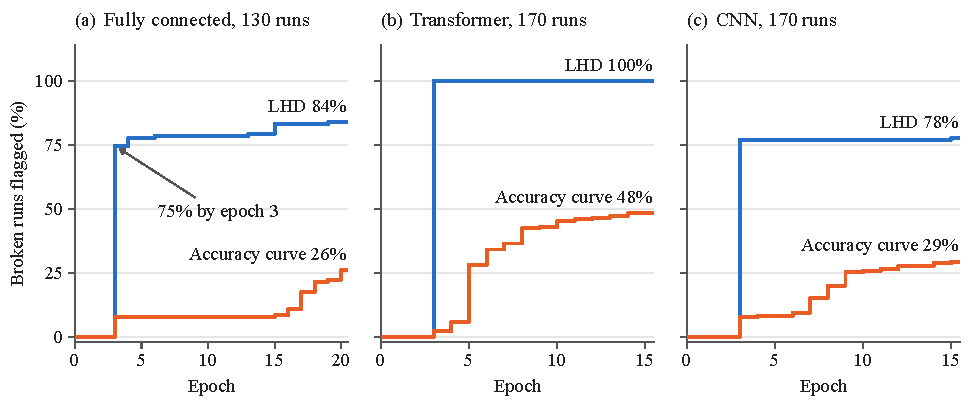
\includegraphics[width=\linewidth]{figures/detection_over_time.pdf}
\caption{Share of broken runs flagged by each epoch, for LHD and the accuracy curve, in each network.}
\label{fig:detection_over_time}
\end{figure}

\section{Every detector}
\label{sec:detectors}

Table~\ref{tab:detectors} lists every detector held to three epochs in a row, with a broken run counted only when the detector named the planted layer. Requiring three epochs instead of one changed little. False alarms did not change, and dead unit catches fell by at most \lhdPatienceDeadChange{}, since a layer's dead unit fraction rarely drops back once it crosses a threshold. Counting only the planted layer mattered more. Counted at any layer, the \lhdSageThreshold{} rule caught more runs with 10\% dead units (\lhdSageAnyTen{}) than with 25\% (\lhdSageAnyTwentyFive{}), because it fired on units that died on their own in other layers. At the planted layer it caught \lhdSageRightTen{} and \lhdSageRightTwentyFive{}.

Two other curve checks did no better than the accuracy curve in the paper. Requiring only one epoch below the healthy range, the accuracy curve caught \lhdAccOneCaught{} broken runs but flagged \lhdAccOneFlagged{} healthy runs. The loss curve, held to three epochs above its range, caught \lhdLossCaught{} and flagged \lhdLossFlagged{}.

\begin{table}[ht]
\centering
\small
\caption{Each detector held to three epochs in a row, with a broken run counted only when the detector named the planted layer. Bold marks the best value in a column when no other detector matches it.}
\label{tab:detectors}
\begin{tabular}{@{}lrrr@{}}
\toprule
 & \multicolumn{2}{c}{Caught at the planted layer} & \\
\cmidrule(lr){2-3}
Detector & Frozen layers & Dead units & Healthy runs flagged \\
\midrule
LHD & 97\% & \textbf{78\%} & 3 of 150 \\
Zero update check & \textbf{100\%} & 0\% & 0 of 150 \\
25\% dead rule & 0\% & 71\% & 51 of 150 \\
SageMaker Debugger (50\%) & 0\% & 40\% & 22 of 150 \\
DeepDiagnosis (70\%) & 0\% & 4\% & 0 of 150 \\
wandb-callbacks (80\%) & 0\% & 0\% & 0 of 150 \\
Any dead unit (wandb-callbacks verbose) & 2\% & 74\% & 100 of 150 \\
\bottomrule
\end{tabular}

\end{table}

\section{Each layer and how many units must die}
\label{sec:layers}

Figure~\ref{fig:per_layer} shows, for every layer and fault, the share of broken runs in which LHD caught the fault and named both the planted layer and the right cause. With 10\%, 25\%, and 50\% of a layer's units dead, LHD caught \lhdDoseALhd{}, \lhdDoseBLhd{}, and \lhdDoseCLhd{} of runs, against \lhdDoseAAcc{}, \lhdDoseBAcc{}, and \lhdDoseCAcc{} for the accuracy curve. It missed some dead unit runs in \lhdDoseMisses{}. In each of these layers, healthy runs already lose a share of units on their own, so the planted fault stayed inside the healthy range. The CNN's dense layer is the clearest case and shows up as the pale row of the figure.

LHD named a layer other than the planted one in \lhdWrongLayerRuns{} caught runs, namely \lhdWrongLayerList{}. In each of them, the layer LHD named had its own signal out of range, so LHD found a real effect of the fault in a different layer. It found the right layer but named the wrong cause in \lhdWrongCauseRuns{} runs, all \lhdWrongCauseList{}. A frozen attention projection also lowers the gradient that reaches it, so its pattern matches a vanishing gradient.

\begin{figure}[ht]
\centering
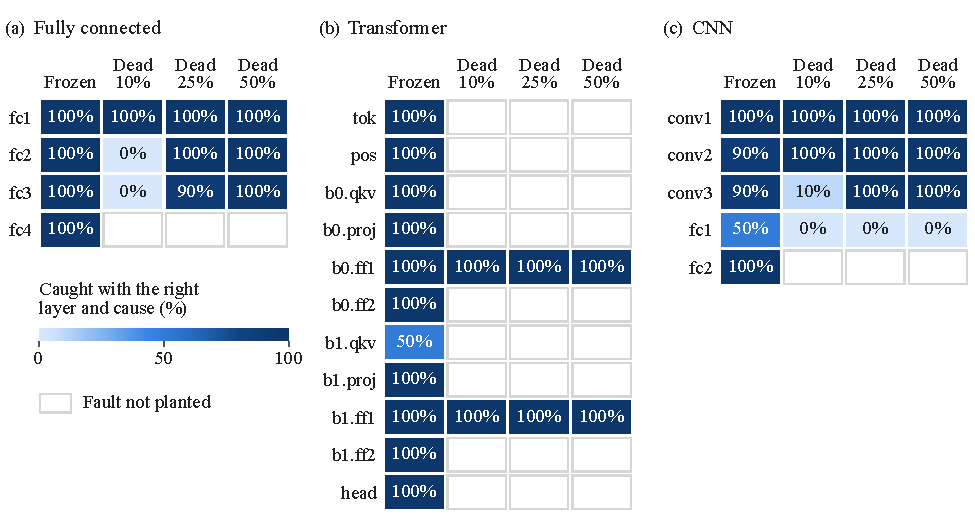
\includegraphics[width=\linewidth]{figures/per_layer.pdf}
\caption{Share of broken runs in which LHD caught the fault and named both the planted layer and the right cause, for every layer and fault. Each cell is \lhdSeedsPerFault{} broken runs. Blank cells are faults that were not planted, since dead units only go into layers followed by a ReLU.}
\label{fig:per_layer}
\end{figure}

\section{What each signal adds}
\label{sec:ablation}

Table~\ref{tab:ablation} replays the same runs with each signal removed or used alone. Without the dead unit fraction, LHD caught \lhdAblationNoDeadCaught{} of broken runs instead of \lhdAblationAllFourCaught{}, so that signal carries most of the detection. Without the weight change, it named the right layer and cause in \lhdAblationNoChangeBoth{} of broken runs instead of \lhdAblationAllFourBoth{}, since the weight change is what separates a frozen layer from other faults. Removing the weight norm or the gradient norm changed little, because none of the planted faults was designed to move them.

\begin{table}[ht]
\centering
\small
\caption{What happens when signals are removed or used alone, pooled over the three networks. Changes are in percentage points against all four signals.}
\label{tab:ablation}
\begin{tabular}{@{}lrrrr@{}}
\toprule
Signals used & \multicolumn{2}{c}{Broken runs caught} & \multicolumn{2}{c}{Right layer and cause} \\
\cmidrule(lr){2-3} \cmidrule(l){4-5}
 & Rate & Change & Rate & Change \\
\midrule
All four & 87\% & & 85\% & \\
\midrule
Without weight change & 70\% & $-$18 & 45\% & $-$40 \\
Without weight norm & 87\% & same & 85\% & same \\
Without grad norm & 87\% & same & 86\% & +1 \\
Without dead unit fraction & 43\% & $-$45 & 41\% & $-$44 \\
\midrule
Only weight change & 43\% & $-$45 & 43\% & $-$42 \\
Only weight norm & 10\% & $-$77 & 0\% & $-$85 \\
Only grad norm & 25\% & $-$63 & 0\% & $-$85 \\
Only dead unit fraction & 52\% & $-$36 & 45\% & $-$40 \\
\bottomrule
\end{tabular}

\end{table}

\section{Margin and calibration size}
\label{sec:settings}

These checks replay the same saved runs and were run after the main results. The settings were fixed before them and were not picked from them. With thresholds right at the edge of the healthy range ($m = 0$), LHD flagged \lhdEdgeFlagged{} of healthy runs and caught \lhdEdgeCaught{} of broken runs. With the margin of \lhdMargin{}, it flagged \lhdMarginFlagged{} and caught \lhdMarginCaught{}. The range also needs enough calibration runs. Table~\ref{tab:calibration} gives the false alarm rate of the worst network when the range is built from fewer runs, averaged over random draws of those runs.

\begin{table}[ht]
\centering
\small
\caption{False alarms when the healthy range is built from fewer calibration runs. Each row shows the network with the highest mean false alarm rate at that size.}
\label{tab:calibration}
\begin{tabular}{@{}rrl@{}}
\toprule
Calibration runs & Healthy runs flagged & Network \\
\midrule
\lhdCalARuns & \lhdCalAWorst & \lhdCalANet \\
\lhdCalBRuns & \lhdCalBWorst & \lhdCalBNet \\
\lhdCalCRuns & \lhdCalCWorst & \lhdCalCNet \\
\lhdCalDRuns & \lhdCalDWorst & \lhdCalDNet \\
\lhdCalERuns & \lhdCalEWorst & \lhdCalENet \\
\lhdCalFRuns & \lhdCalFWorst & \lhdCalFNet \\
\bottomrule
\end{tabular}
\end{table}

\section{Cost}
\label{sec:cost}

Monitoring added \lhdMlpOverhead{} to the training time of the fully connected network, \lhdTransformerOverhead{} for the transformer, and \lhdCnnOverhead{} for the CNN, measured on fresh healthy runs on one CPU thread. Most of that time goes to the gradient norm, read after every batch, and to the probe batch, run once per epoch, so the overhead is largest for the network with the cheapest epochs. Stopping each broken run at LHD's alarm would have saved \lhdComputeSaved{} of its training on average. All runs together took \lhdTrainingHours{} hours of CPU time on one laptop.

\section{Faults beyond frozen layers and dead units}
\label{sec:extra}

A third set of runs tested faults the rules were not built around (Table~\ref{tab:extra}). It was planned with the rest and trained after the main results were in. Two of these faults are the main ones started at epoch \lhdLateOnset{} instead of epoch 1, a frozen layer and half of a layer's units killed. A gradient cut detaches the input of one layer from the first epoch, so that layer and the ones after it keep learning while no gradient reaches the layers before it. A learning rate jump multiplies Adam's learning rate by 10 or 100 at the start of epoch \lhdLateOnset{}. The cosine schedule keeps shrinking the rate from the raised value, so in the \lhdCnnEpochs{} epoch networks, epoch \lhdLateOnset{} trains at \lhdLrTimesTen{} or \lhdLrTimesHundred{} instead of \lhdLrNormal{}.

LHD caught \lhdLateFrozenCaught{} of \lhdLateFrozenRuns{} late frozen layers and named the layer and cause in \lhdLateFrozenBoth{}, while the accuracy curve caught \lhdLateFrozenAcc{}. It caught \lhdLateDeadCaught{} of \lhdLateDeadRuns{} runs with half a layer's units killed late and named the layer and cause in \lhdLateDeadBoth{}. It caught \lhdCutCaught{} of \lhdCutRuns{} gradient cuts, named a layer before the cut in \lhdCutBoth{}, and called the cause a vanishing gradient, which is the only test of that rule. LHD also fired on every learning rate jump, but the causes it named were mixed. For a tenfold jump it named \lhdLrTenCauses{}, and for a hundredfold jump it named \lhdLrHundredCauses{}. No run produced a value that was not a finite number, so the divergence rule never fired.

The zero update check caught every late frozen layer. Held to three epochs it fired in the same epoch as LHD in \lhdLateZeroTies{} runs, and when one epoch is enough it fires at epoch \lhdLateZeroEpoch{}. It also caught \lhdCutZero{} gradient cuts, since the layers before a cut never move. The \lhdSageThreshold{} rule caught \lhdLateDeadSage{} late half dead runs at the planted layer, while flagging \lhdSageFlagged{} of \lhdHealthyRuns{} healthy runs.

\begin{table}[ht]
\centering
\small
\caption{Faults beyond the main study, pooled over the three networks. Every detector is held to three epochs in a row. The zero update check and the \lhdSageThreshold{} dead rule count a run only when they name the planted layer, or a layer before a gradient cut, and any alarm counts for a learning rate jump, which has no planted layer. Bold marks the best value in a row when no other detector matches it.}
\label{tab:extra}
\begin{tabular}{@{}lrrrrr@{}}
\toprule
 & & & Accuracy & Zero update & 50\% dead \\
Fault & Runs & LHD & curve & check & rule \\
\midrule
Frozen layer at epoch 6 & 100 & 100\% & 20\% & 100\% & 0\% \\
50\% dead units at epoch 6 & 45 & \textbf{89\%} & 16\% & 0\% & 82\% \\
Gradient cut & 30 & 100\% & 100\% & 100\% & 0\% \\
Learning rate $\times 10$ at epoch 6 & 15 & \textbf{100\%} & 33\% & 0\% & 0\% \\
Learning rate $\times 100$ at epoch 6 & 15 & 100\% & 100\% & 67\% & 60\% \\
\midrule
Healthy runs flagged & 150 & 3 & 7 & \textbf{0} & 22 \\
\bottomrule
\end{tabular}

\end{table}

\section{Statistics for each seed and condition}
\label{sec:stats}

Averaged within each seed, all \lhdSeedGroups{} seed groups favored LHD (\lhdSeedP{}), which is the most extreme result a one sided Wilcoxon test can give with that many groups. Averaged within each fault condition, \lhdConditionsLHD{} of \lhdConditions{} conditions favored LHD (\lhdConditionP{}). Of the others, neither detector fired in \lhdConditionsNeither{}, both fired at the same epoch in \lhdConditionsSame{}, and the accuracy curve was earlier in \lhdConditionsAcc{}, \lhdConditionsAccWhere{}. Counting a run the accuracy curve never caught as one epoch past its end, the mean gap over all broken runs was \lhdMeanGapAll{} epochs (95\% interval \lhdMeanGapInterval{} from the bootstrap over seeds). That figure leans on the runs the accuracy curve missed, so the gap on runs both caught, reported in the paper, is the fairer measure.

\end{document}
